\documentclass[table]{beamer}
\usepackage[german]{babel}

\usepackage{tikz}
\usetikzlibrary{positioning,
                calc,
                decorations.pathreplacing,
                calligraphy}
\usepackage{tikzscale}
\usepackage{libertine}
\usepackage{pgf-pie}
\usepackage{hyperref}
\usepackage{booktabs}
\usepackage{diagbox}
\usepackage{xcolor}

\title{Versionskontrolle von Texten}
\subtitle{Git und GitHub}
\date{1. Februar 2024}

\begin{document}
    \frame{\titlepage}

    \begin{frame}
        \frametitle{Wichtige Quellen}
        \begin{itemize}
            \item git-scm.com
            \item docs.github.com/decorations
            \item code.visualstudio.com/docs/sourcecontrol/overview
        \end{itemize}
    \end{frame}

    \begin{frame}
        \frametitle{Ausgangslage}
        Wer kennt das nicht?

        \vspace*{5mm}

       \only<2>{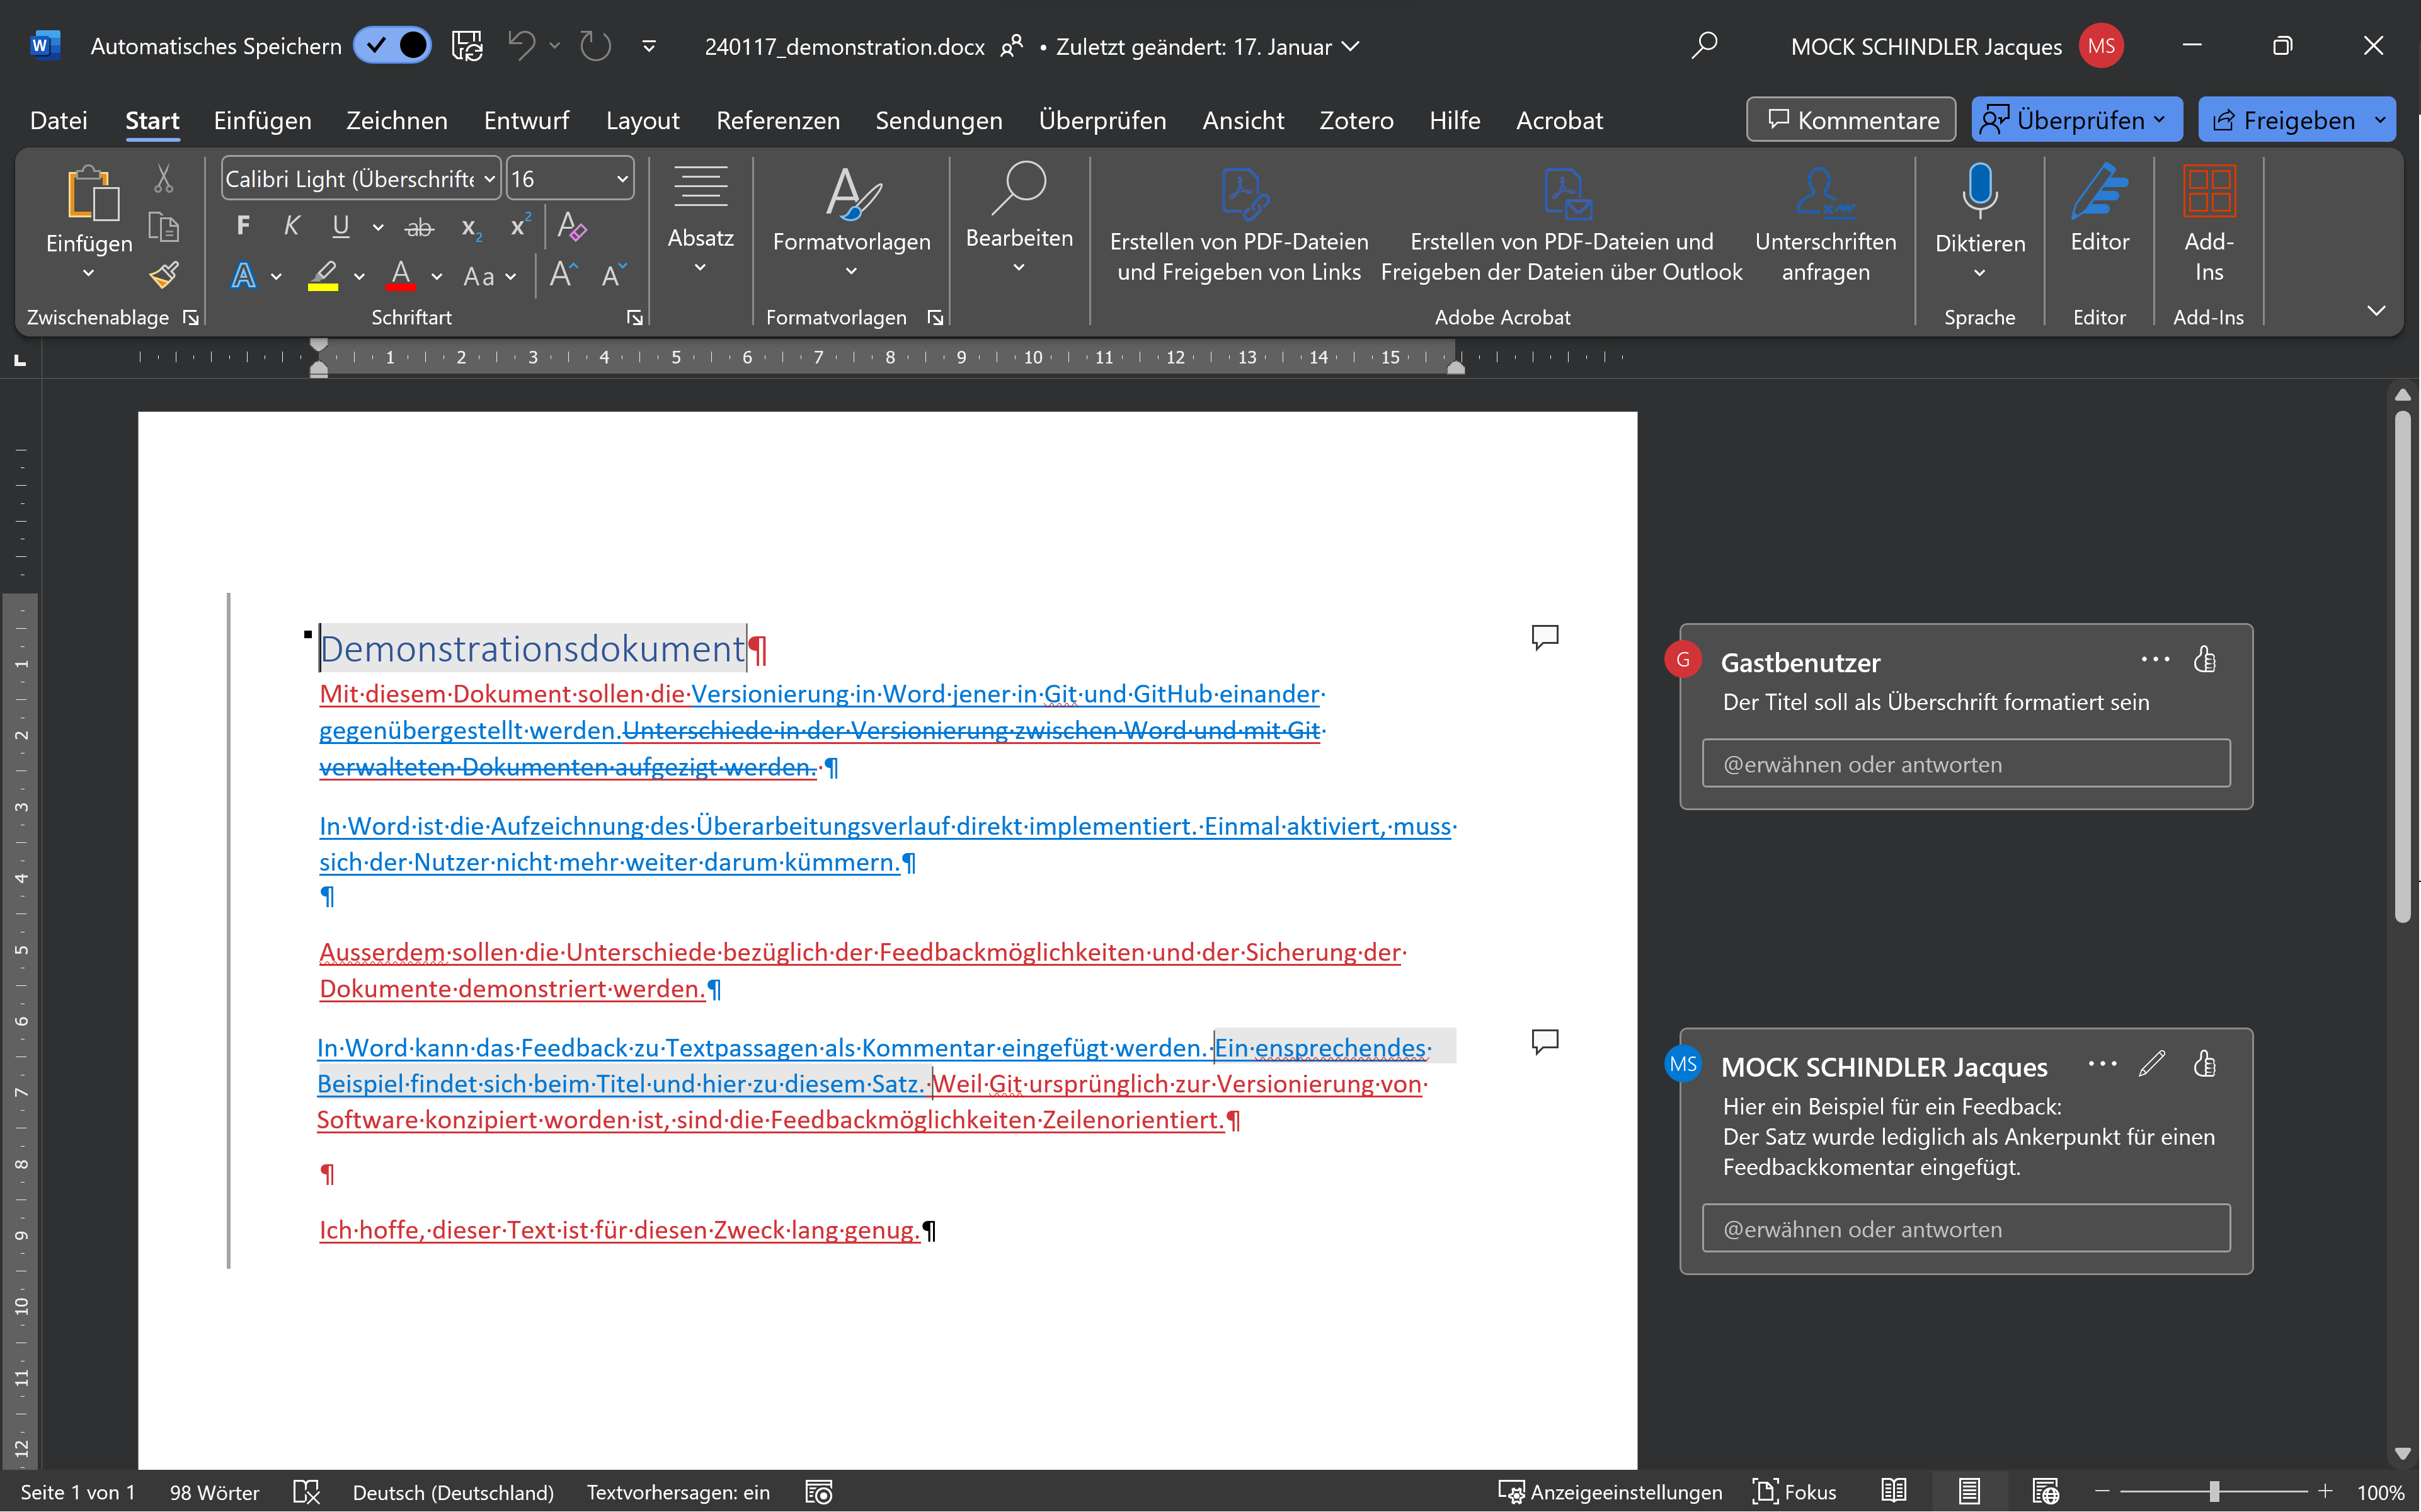
\includegraphics[width=\textwidth]{images/word_markup.png}} 
       \only<3>{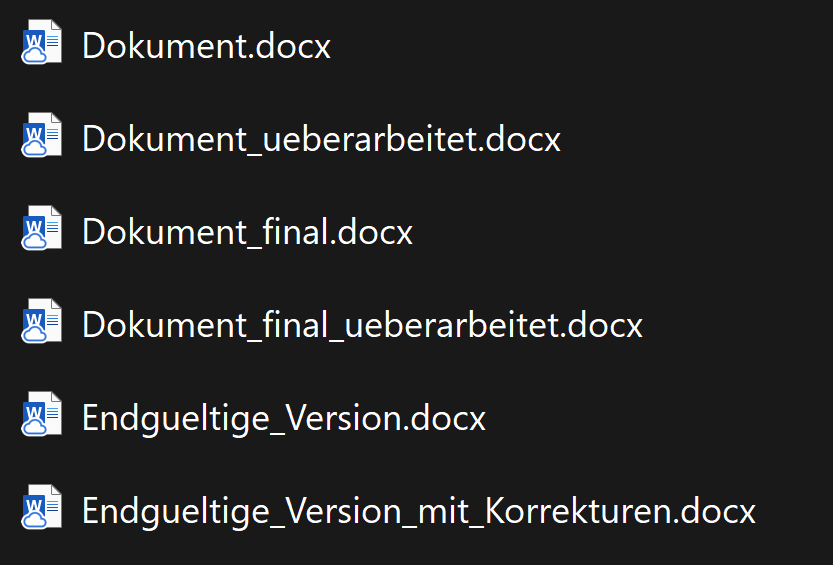
\includegraphics[width=\textwidth]{images/file_manager.png}}
    \end{frame}

    \begin{frame}
        \frametitle{Ausgangslage}
        Das hoffentlich nicht, aber wer weiss?

        \vspace*{5mm}

       \visible<2>{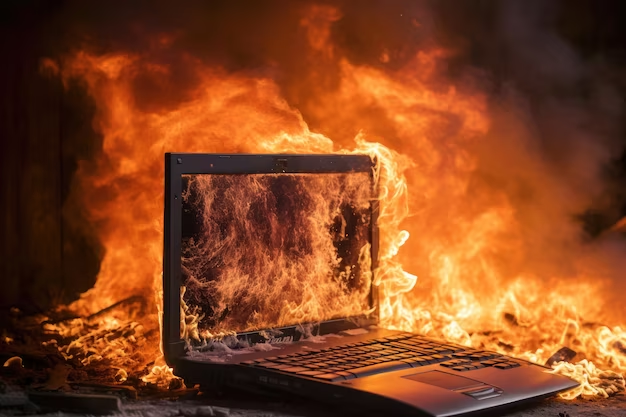
\includegraphics[width=\textwidth]{images/burning_laptop.png}} 
       
    \end{frame}

    \begin{frame}
        \frametitle{Warum Versionierung}

        \begin{itemize}
            \item Back-up
            \item just one source of truth
            \item transparente Textgenese
        \end{itemize}
    \end{frame}

    \begin{frame}
        \frametitle{Back-up}

        \begin{itemize}
            \item lokales Back-up
                
            nicht so sicher -- insbesondere im Falle eines Velusts des
            Computers
            
           \item Back-up in der Cloud
           \begin{itemize}
            \item GitHub
            \item GitLab
            \item GitBucket
            \item Azure Repos
            \item \dots
           \end{itemize}
        \end{itemize}   
        
    
    \end{frame}

    \begin{frame}
        \frametitle{just one source of truth}

        \visible<overlay specification>{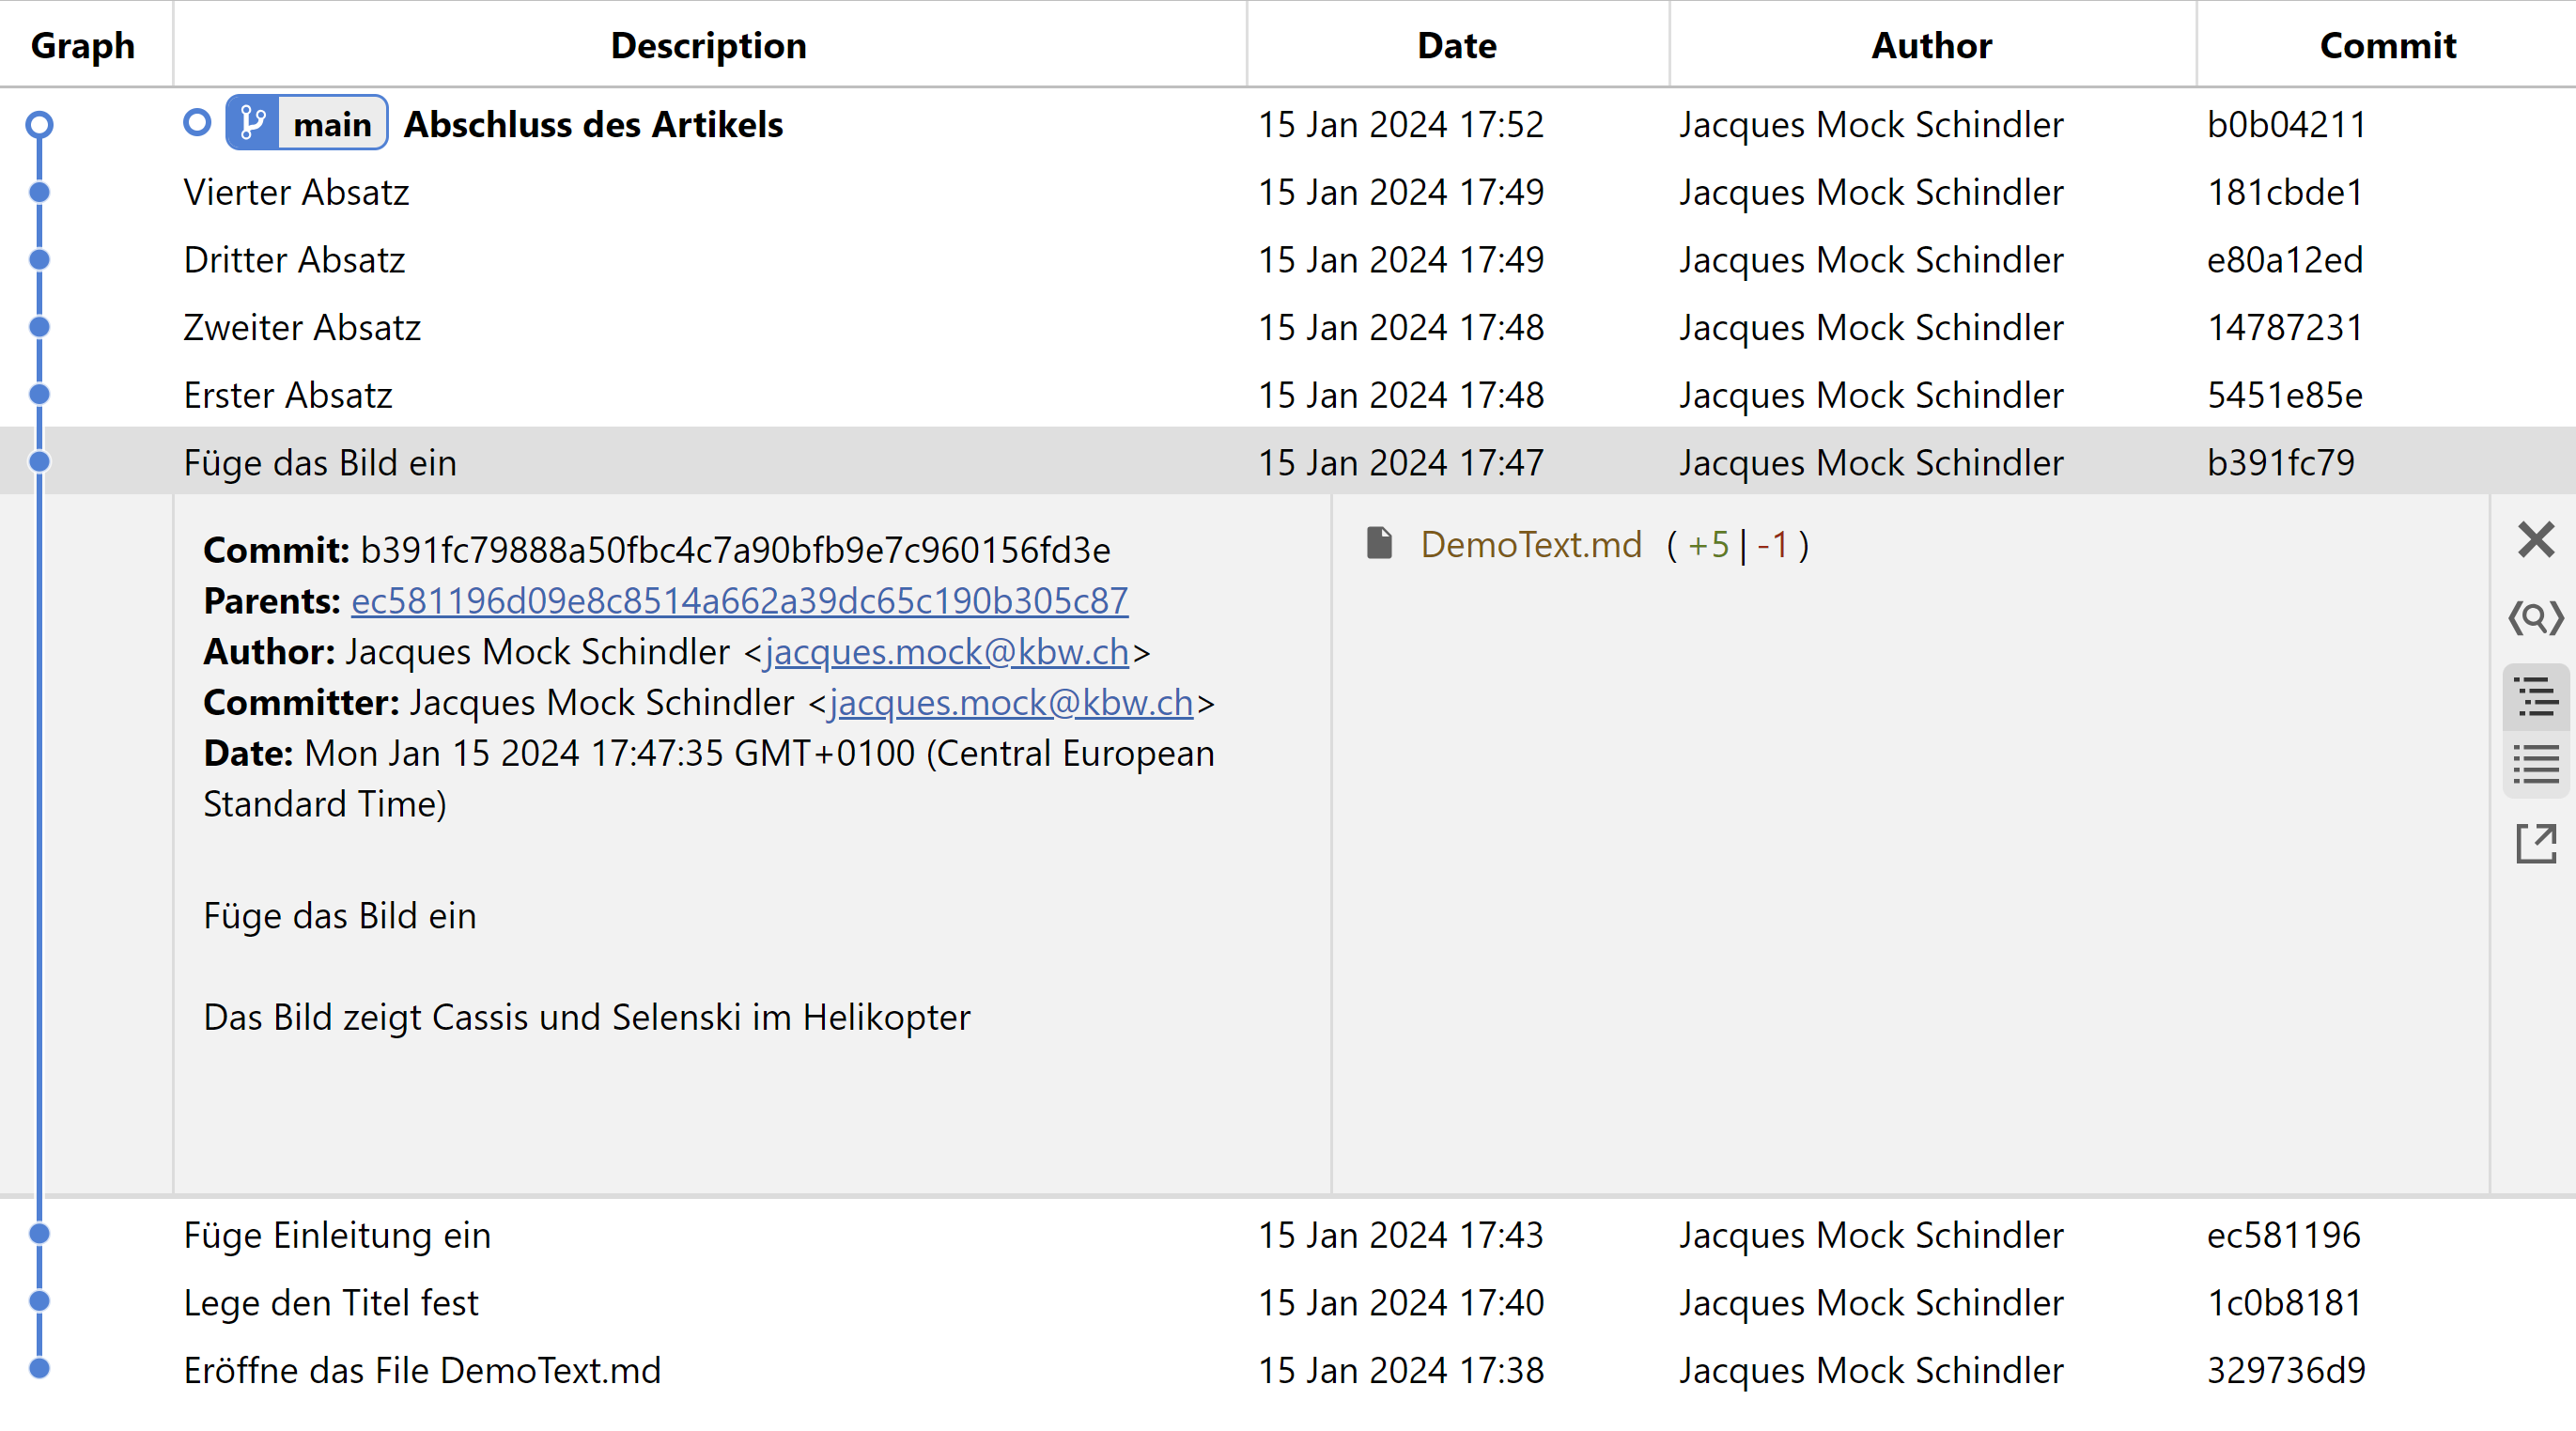
\includegraphics[width=\textwidth]{images/git_graph_details.png}}
  
        
    
    \end{frame}

    

\end{document}
